\chapter{GPU and Clock Unit design}

TODO: intro chaptitre ici

\section{GPU}
The GPU bears its name rather badly because it is not really programmable. This unit provides a 
graphic memory and the tools to draw patterns, called masks of 8x8 pixels. The writing in this 
memory is done from the beta machine (the CPU) through the instruction store (ST). The specific way 
of addressing the memory and the structure of the commands, passed through the data line of the 
store, are described later. As far as the colors are concerned, it has been decided to work with 
12bit RGB colors, that is to say 4 bits per color.

In addition to this, the GPU also provides the HDMI controller. This controller simply reads the 
graphics memory in a loop and draws its content on the screen. The controller can thus handle a 
16:9 screen with a resolution of 848x480 pixels and a refresh rate of 60Hz. The protocol used is 
the VESA 848x480, it is described later. 

Before moving on to the description of the different modules making up the GPU, a description of 
how the screen and the masks are interpreted by the GPU is done.

\subsection{Screen and tiles representation}

As said before, the masks are 8x8 pixels and the goal is to be able to apply them to the screen. 
The screen is therefore naturally divided into a set of 8x8 pixel squares which are called tiles. 
In memory, the idea is that there are 3 sub-memories whose words contain a color of the three 
primary colors (red, green or blue) of a whole tile. A tile corresponding to 64 pixels and a 
primary color being coded on 4 bits, it gives words of 256 bits. Then, by dividing the dimensions 
of the screen (848x480 pixels) by 8, we find that 106x60 tiles, so 6360 are enough to represent 
the screen. In order not to use too much memory, it is decided to use 72x54 tiles. This corresponds 
to the largest integer size allowing a 4:3 ratio with a maximum use of 4096 tiles.  It is decided 
to limit to 4096 tiles because to use 6360 tiles it would be necessary to have a memory with 8192 
words, which would use too much memory unnecessarily. The useful screen is centered in the physical 
screen. Figure \ref{fig:gpu/screen_size} summarizes all this.

\begin{figure}[H]
    \centering
    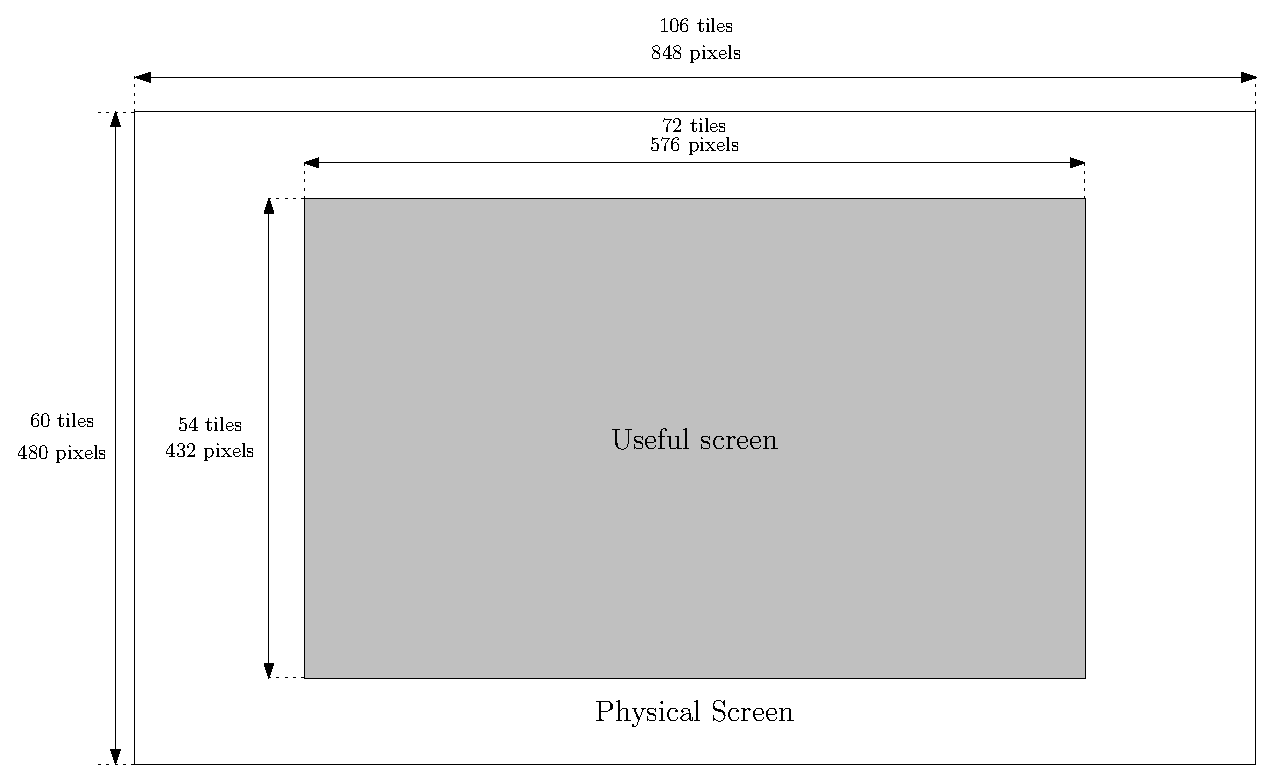
\includegraphics[width=\linewidth]{Chapter4-GPU_CLKU/res/screen_size}
    \caption{Useful screen area in the physical screen}
    \label{fig:gpu/screen_size}
\end{figure}

The problem with putting all tiles in a single memory like this is that only one tile is accessible 
at a time. This means that a mask can only be applied to one tile. This is a pity because it 
prevents the mask from being drawn anywhere on the screen. Indeed, the mask cannot for example be 
drawn between two tiles as shown in Figure \ref{fig:gpu/mask_2tiles}.

\begin{figure}[H]
    \centering
    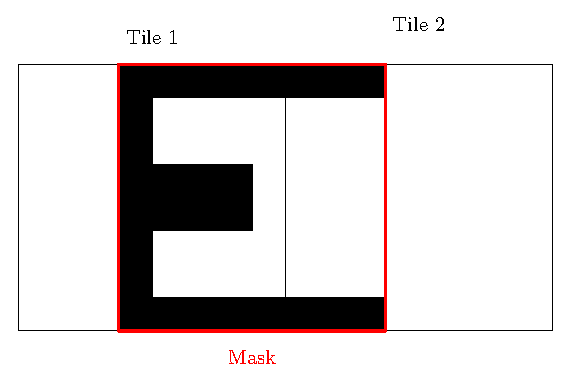
\includegraphics[scale=1.0]{Chapter4-GPU_CLKU/res/mask_2tiles}
    \caption{Mask overlapping two tiles}
    \label{fig:gpu/mask_2tiles}
\end{figure}

When such a placement of the mask takes place, what actually happens is a tile is chosen first. And 
then an offset in pixels is added to the mask. In the example in Figure, the mask has a positive 
offset of N pixels with respect to Tile 1. The idea is then to allow a mask to have an offset 
ranging from 0 to 7 depending on the abscissa and ordinate. It is not useful to go further than 7 
as this corresponds to placing the mask at the next tile. To be able to apply the mask, it is 
therefore necessary to be able to load four tiles. The first one being the one chosen to draw the 
mask in (x, y), the others being those in (x + 1, y), (x, y + 1) and (x + 1, y + 1). A naive 
solution to load these four tiles would be to have a memory for each tile. However, this has two 
problems. The first is that this is impossible for the Cyclone V. Indeed, it was seen earlier that 
the Cyclone V has just over 500 M10K memory blocks. However, to represent all the tiles, we would 
need 3888 memories because the definition of a memory must use at least one whole M10K, which is 
simply impossible. 

Another way is to try to divide the set of tiles into four groups. These four groups should be 
distributed on the screen in such a way that the placement of a mask loads 4 tiles of different 
groups each time. If one thinks about it, it is possible to convince itself that a simple paving 
of 4 colors allows this (a color represents a group). Figure \ref{fig:gpu/screen_tiling} shows such 
a tiling. 

\begin{figure}[H]
    \centering
    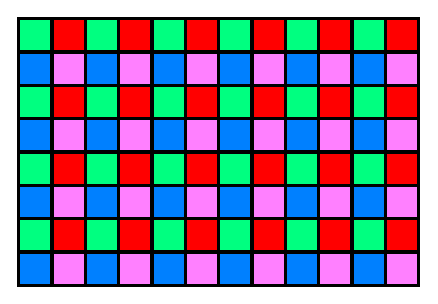
\includegraphics[scale=1.0]{Chapter4-GPU_CLKU/res/screen_tiling}
    \caption{Screen tiling}
    \label{fig:gpu/screen_tiling}
\end{figure}

And the different cases possible by choosing four tiles in the way explained earlier, i.e. one 
tile, the one to the right of it, the one below it and the one at the bottom right are shown 
Figure \ref{fig:gpu/screen_tiling_cases}. It can be seen that in each case, a group is present only 
once, which validates the possibility of representing all tiles in four distinct memories.

\begin{figure}[H]
    \centering
    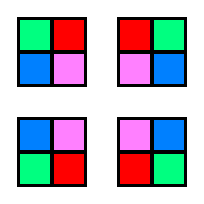
\includegraphics[scale=1.0]{Chapter4-GPU_CLKU/res/screen_tiling_cases}
    \caption{Screen tiling selection cases}
    \label{fig:gpu/screen_tiling_cases}
\end{figure}

\subsection{Mask representation}

A mask has the same dimensions as a tile but does not have the same content. Indeed, a mask can 
contain four different values. The first value is keep, corresponding to a 0 in the mask. This 
value means that no modification will be made to the pixel screen targeted by this position in the 
mask. Then there is the set primary, corresponding to the value 1 which will set the pixel at this 
location to the primary color which will be defined in the set instruction, we will come back to 
this later. When the value is 2, it is then a so-called secondary color that is applied. And 
finally, the value 3 corresponds to a reset, the pixel then becomes black. Each of these values 
can therefore be represented on 2bits. Table \ref{tab:mask_op} summarizes the possible operations
of a mask. 

\begin{table}[H]
    \centering
    \begin{tabular}{|l|c|}
    \hline
    \rowcolor[HTML]{DAE8FC} 
    \multicolumn{1}{|c|}{\cellcolor[HTML]{DAE8FC}\textbf{Mask Operation}} & \textbf{Mask Value} \\ \hline
    Keep                                                                  & 0b00                \\ \hline
    Set primary                                                           & 0b01                \\ \hline
    Set secondary                                                         & 0b10                \\ \hline
    Reset                                                                 & 0b11                \\ \hline
    \end{tabular}
    \caption{Mask operations}
    \label{tab:mask_op}
\end{table}

In terms of representation, a mask is a simple vector of 8x8x2 (128) bits. Its LSB corresponds to 
the upper left corner of the mask and its MSB corresponds to the lower right corner of the mask. 
This correspondence is shown in Figure \ref{fig:gpu/mask_vector}.

\begin{figure}[H]
    \centering
    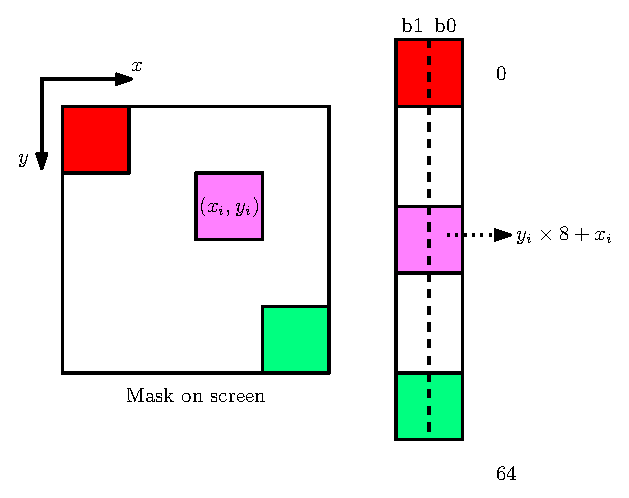
\includegraphics[scale=1.0]{Chapter4-GPU_CLKU/res/mask_vector}
    \caption{Mask vector representation}
    \label{fig:gpu/mask_vector}
\end{figure}

\subsection{Using the GPU}

As introduced, to use the GPU, it is necessary to use the store instruction from the CPU. But the 
address and data must be correctly formatted. For the address, it must start with 0b10 as seen in 
the chapter on the CPU (so that the addressed unit is the GPU). Then, it was decided to make the 
address natural, that is to say that it is 
readable without any conversion. The address therefore contains the exact pixel position where 
a mask should be applied. A pixel being located by four variables: block\_x, block\_y (corresponding 
to the tile), off\_x and off\_y (corresponding to the offset from the tile), these four variables 
are directly present in the address. The format of the address is explained in 
Figure \ref{fig:gpu/store_address}.

\begin{figure}[H]
    \centering
    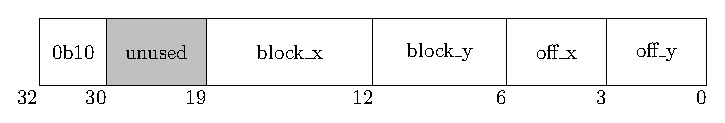
\includegraphics[scale=1.0]{Chapter4-GPU_CLKU/res/store_address}
    \caption{Store instruction address}
    \label{fig:gpu/store_address}
\end{figure}

Concerning data, it must contain the mask identifier and the values of the two colors. As a color is 
represented on 12 bits and a word on the CPU is represented on 32 bits, 8 bits remain for the mask.  
The GPU can therefore support 256 masks. The data format is detailed in 
Figure \ref{fig:gpu/store_data}.

\begin{figure}[H]
    \centering
    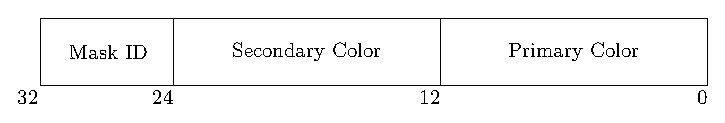
\includegraphics[scale=1.0]{Chapter4-GPU_CLKU/res/store_data}
    \caption{Store instruction data}
    \label{fig:gpu/store_data}
\end{figure}